\documentclass{beamer}

%%%%%%%%%%%%%%%%%%%%%%%%%%%%%% Loading packages that alter the style
\usepackage[farmed, numberded]{graphicx}
\usepackage[]{color}
\usepackage{alltt}
\usepackage[T1]{fontenc}
\usepackage[utf8]{inputenc}
\usepackage{dirtytalk}
\usepackage{ragged2e}
\usepackage{amssymb}
\usepackage{amsmath}
\usepackage{amsthm}
\usepackage{amsfonts}
\usepackage{amssymb}
\usepackage{physics}
\usepackage{listings}
\usepackage{epigraph} 
\usepackage{blindtext} %This package generates automatic text
\usepackage[framed, numbered]{matlab-prettifier}
\setcounter{secnumdepth}{3}
\setcounter{tocdepth}{3}
\setlength{\parskip}{\smallskipamount}
\setlength{\parindent}{0pt}
\newtheorem{teo}{Teorema}[section]
\newtheorem{coro}{Corolario}[subsection]
\newtheorem{prop}{Proposición}[subsection]
\newtheorem{dfn}{Definición}
\newtheorem{examp}{Ejemplo}
\usetheme{Boadilla}
\usepackage{lipsum}
\usepackage{hyperref}
\hypersetup{hidelinks,linkcolor = black}
\usepackage{listings}

\raggedbottomhttps%://www.overleaf.com/project/61a28f32cde4ed5c68942eea

\newcommand\Fontvi{\fontsize{6}{7.5}\selectfont}

%%%%% Portada %%%%%%%
\title[Advanced MicroEconometrics]
{Estimating the Return to Schooling: Progress on Some Persistent Econometric Problems}

\author[Luis Martínez] 
{Luis Gerardo Martínez Valdés}
\institute{ITAM}
\date{Spring 2022}
\logo{\includegraphics[height=.5cm]{itamlogo.png}}
%%%%%%%%%%%%%%%%%%%%%%%%%%%%%%%%

\begin{document}

\frame{\titlepage}

\begin{frame}{Table of Contents}
\Fontvi
\tableofcontents
\end{frame}

%%% Sintaxis de las diapositivas %%%%%%
\section{Objetive}
\begin{frame}{Objective}
 \begin{itemize}
     \item To measure the \textbf{causal effect of education} on \textcolor{red}{labor market earnings} by using institutional features of the \textcolor{blue}{supply side} of educations system as an exogeneous determinants of schooling outcomes.
     
 \begin{block}{Key Finding}
Author made a review of studies that have used compulsory schooling laws, differences in the accessibility of schools, and similar features as \textbf{IVs} for completed education, reveals that the resulting estimates of the return to schooling are typically as big or bigger than the corresponding \textbf{OLS'} estimates.
\end{block}

    \item We will give a few explanations or interpretations (if you will) of why this happens.
 \end{itemize}
\end{frame}



\section{Introduction}
\subsection{Background}
\begin{frame}{Background}

   \begin{itemize}
       \item Resurgence of interest in the study of causal links between education and labor market success. 
       \item Qualified vs Under-Qualified Workers.
       \item Revival in the determinants of economic growth.
       \item New focus on the role of human capital.
       \item Concerns about the relative costs and benefits of higher education for those who were not previously receiving it.
   \end{itemize}
   
   
\end{frame}

\subsection{Introduction}
\begin{frame}{Introduction}
Institutional features of the education system and supply-side variables. 
\begin{itemize}
    \item How are they used? 
    \item Why? 
    \item What is their impact today?
\end{itemize}

\begin{block}{Aim}
Card aims to present a present a survey and partial synthesis of the recent literature that has used \say{supply-side} features of the education system to help identify the causal effect of education. By doing this, he will try to reconcile various findings in the literature, and also provide a useful framework for generating new hypotheses and insights about the connection between education and earnings.
\end{block}
   
\end{frame}

\subsection{Structure}
\begin{frame}{Structure}
\begin{itemize}
    \item Presentation of simple theoretical model of endogenous schooling.
    \item Use this model to to motivate an extended discussion of various econometric issues.
    \item Present a selective review of the recent literature on estimating the economic returns to education, drawing on studies of the U.S. and other developed economies, as well as a handful of studies of developing economies.
\end{itemize}
    
\end{frame}

\section{A Model of Endogenous Schooling}
\subsection{Framework}
\begin{frame}{Framework}
    Card builds on Becker's (1967) model of endogenous schooling, since most conceptual issues underlying the interpretation of recent studies of the return to education can be illustrated in the framework presented by the latter. 
    
    \begin{itemize}
        \item Individuals face a market opportunity locus that gives the level of earnings associated with alternative schooling choices. 
        \item Thus, they reach an optimal schooling decision by balancing the benefits of higher schooling against the costs.
    \end{itemize}
    
    \begin{block}{Strong Assumption}
        Traditionally, it is assumed that individuals seek to maximize the discounted present value of earnings, net of schooling costs

    \end{block}

\end{frame}
\subsection{Model}
\begin{frame}{Model}
    \begin{itemize}
        \item Assume that individuals have an infinite planning horizon that starts at the minimum school-leaving age ($t=0$). 
        \item They accumulate a flow of utility in period $t$ that depends on:
        \begin{itemize}
            \item consumption $c(t)$ at period $t$
            \item Wether they are in school (and working part time) or out of school and working full time. 
        \end{itemize}
        \item \textbf{Utility while in school is}:
                        \begin{equation*}
                                u(c(t))-\phi(t)
                        \end{equation*}
        \item \textbf{Utility out of school is}:
                        \begin{equation*}
                                u(c(t))
                        \end{equation*}
    \end{itemize}
    
\end{frame}

\begin{frame}{}
    \begin{block}{Note:}
        Note that $u(\cdot)$ is an increasing concave function and $\phi(t)$ is a convex function that represents \textcolor{blue}{relative disutility of school vs. work for the t-th year of schooling}.
    \end{block}
 Finally, 
 \begin{itemize}
     \item Individuals discount future utility flows at a subjective discount rate $\rho$, and make a once-for-all decision on when to leave school.
 \end{itemize}
 
 Therefore, one can define \textbf{lifecycle utility, conditional on schooling $S$} and a given consumption profile as
 \begin{equation*}
     V(S,c(t))=\int_{0}^{S}\Big[ u(c(t)-\phi(t))\Big]e^{-\rho t} dt + \int_{S}^{\infty}u(c(t))e^{-\rho t} dt
 \end{equation*}
 
\end{frame}

\begin{frame}{Intertemporal Budget Constraint}
\begin{itemize}
    \item Let $y(S,t)$ denote real earnings at age $t$ of an individual who has completed $S$ years of post-compulsory schooling (with $0\leq S \leq t$).
    \item Assume that individuals who are in school at time $t$ work part time and earn $p(t)$ and pay tuition costs of $T(t)$. 
    \item Also, assume that individuals can borrow or lend freely at a \textbf{fixed} interest rate R. 
\end{itemize}

Thus, we can define the \textbf{intertemporal budget constraint}: 
\begin{equation*}
    \int_{0}^{\infty}c(t)e^{-Rt}dt= \int_{0}^{S}\Big[ p(t)- T(t)\Big]e^{-R t} dt + \int_{S}^{\infty}y(S,t)e^{-R t} dt
\end{equation*}

\end{frame}

\begin{frame}{Optimal Schooling choice and Optimal Consumption Path}

Therefore, an individual’s optimal schooling choice and optimal consumption path maximize
\begin{align*}
    \Omega(S,c(t),\lambda) &  =  V(S,c(t)) \\
                           &  - \lambda \Bigg[ \int_{0}^{\infty}c(t)e^{-Rt}dt~- \int_{0}^{S}\Big[ p(t)- T(t)\Big]e^{-R t} dt \\
                           &  - \int_{S}^{\infty}y(S,t)e^{-R t} dt \Bigg]\\
\end{align*}

We can see that the FOC with respect to $S$ yields:
\begin{equation*}
    \Omega_{S}(S,c(t),\lambda)=\lambda e^{-RS}[MB(S)-MC(S)]
\end{equation*}
\end{frame}

\begin{frame}{}
    Where, 
    \begin{itemize}
        \item The Marginal Benefit of the $S$-th unit of schooling is defined by
        \begin{equation*}
            MB(S) = \int_{0}^{\infty} \frac{\partial y(S,S+\tau)}{\partial Se^{-R \tau}} d \tau
        \end{equation*}
        \item And, the Marginal Cost of $S$-th unit of schooling is given by
        \begin{equation*}
            MC(S) = y(S,S) - p(S) + T(S) +\frac{1}{\lambda e^{-(\rho - R)S}}\phi(S)
        \end{equation*}
    \end{itemize}
\begin{block}{What happens if $MC(S)$ rises faster than $MB(S)$ ?} 
We would need a necessary and sufficient condition for the optimal schooling choice $S$, i.e. $MC(S)=MB(S)$
\end{block}
\end{frame}

\begin{frame}{}
Card solves this problem by assuming that log earnings are additively separable in education and years of post-schooling experience. Therefore, one can write the earnings function as $y(S,t)= f(S)h(t-S)$ (recall that $0 \leq S \leq t$), then 
\begin{equation*}
    MB(S)= f'(S) \int_{0}^{\infty} h(\tau) e^{R \tau}d\tau \equiv f'(S) H(R)
\end{equation*}
 
 where $H(R)$ is a decreasing function of the interest rate. Therefore, 2 conclusions arise: 
 \begin{enumerate}
     \item If earnings are fixed after completion of schooling: $H(R)=\frac{1}{R}$
     \item If earnings follow a \textit{concave} lifecycle profile and taking g as a constant growth rate(equivalent to the lifecycle profile): $H(R)=\frac{1}{(R-g)}$
     
 \end{enumerate}
 
 Therefore, under separability(check Minkowski's Theorem), the marginal costs and benefits of additional schooling are equated when
 \begin{equation*}
     \frac{f'(S)}{f(S)}= \frac{1}{H(R)}\Bigg[ 1+ \frac{(T(S)-p(S))}{f(S)} + \frac{1}{\lambda e^{-(\rho - R)S}}\frac{\phi(S)}{f(S)}\Bigg]
 \end{equation*}
\end{frame}

 \begin{frame}{General Case: $U(c(t)) = log[c(t)]$}
     The FOC's for an optimal consumption profile, together with the lifecycle budget constraint, imply that
     \begin{equation*}
         \frac{1}{\lambda}= \rho \Bigg\{ e^{-RS}f(S) H(R) + \int_{0}^{S} \Big[ p(t) -T(t)\Big] e^{-R t} dt \equiv \rho W(S) \Bigg\}
     \end{equation*}
     
where $W(S)$ is the value of lifecycle wealth associated with the schooling choice S. If $T(S) \approx p(S)$ then 
\begin{equation}
    \frac{f'(S)}{f(S)}= R - g +\rho e^{-\rho S}\phi(S) \equiv d(S)
\end{equation}

\begin{block}{Observations}
 The interest rate must be adjusted to reflect lifecycle earnings growth and the marginal cost has to account for the relative disutility of attending the Sth year of schooling.

\end{block}
\end{frame}  

\begin{frame}{Heterogeinity in the Optimal Schooling Choice}
    Individual heterogeinity can arise from 2 sources: 
    \begin{enumerate}
        \item differences in the economic benefits of schooling,
        \item differences in the marginal costs of schooling.
    \end{enumerate}
    
Then we would have 
% Equation 2
\begin{equation}
    \frac{f'(S)}{f(S)}= b_{i} - k_{1}S,~~~ k_{1}>0
\end{equation}
%Equation 3
\begin{equation}
    d(S) = r_{i} + k_{2}S, ~~~k_{2}>0
\end{equation}

where $b_{i}\sim F(\bar{b},\sigma_{b}^{2})$, $r_{i}\sim F(\bar{r},\sigma_{r}^{2})$. Equating (2) with (3) and solving for $S$ will yield, 
%Equation 4
\begin{equation}
    S_{i} =(b_{i}-r_{i})/k,~~~k=(k_{1}+k_{2})>0
\end{equation}

\end{frame}

\begin{frame}{}
At the equilibrium level of schooling described by equation (4) individual i’s marginal return to schooling is
\begin{equation*}
    \beta_{i} \equiv b_{i} - k_{1}S = b_{i}(1-\frac{k_{1}}{k}) + r_{i}\frac{k_{1}}{k}
\end{equation*}

The average marginal return to education is therefore, 
\begin{equation*}
    \bar{\beta} = \mathbb{E}[\beta_{i}]= \mathbb{E}[b_{i}-k_{1}S]= \bar{b} + k_{1}\bar{S}
\end{equation*}

\begin{block}{Interpretation of equation (4)}
 Card interprets (4) as partial equilibrium description of the relative education choices of a cohort, given the institutional environment and economic conditions that prevailed during their late teens and early twenties.
\end{block}
\end{frame}


\section{Econometric Issues Raised By Endogenous Schooling}
\subsection{OLS Estimates of the Return to Schooling}
\begin{frame}{Econometric Issues Raised By Endogenous Schooling: OLS Estimates of the Return to Schooling}
Note that equation (2) implies a model for log earnings of the form 
%%%% EQUATION 5
    \begin{equation}
        log~y_{i}= a_{0} + \bar{b}S_{i}-\frac{1}{2}k_{1}S_{i}^{2} + a_{i} + (b_{i}-\bar{b})S_{i},
    \end{equation}

where $a_{i} \equiv \alpha_{i}-a_{0}$ has mean $0$. Together with some algebraic manipulation andconsidering the linear projectos of the underlying random variables $a_{i},~~~ b_{i}$ and $r_{i}$, one can rewrite expression (5) as 

 \begin{equation}
        log~y_{i}= K + (\bar{b}+\lambda_{0}-\psi_{0}\bar{S})S_{i} + (\psi_{0} - \frac{1}{2}k_{1})S_{i}^{2} + u_{i} + v_{i}S_{i},
    \end{equation}
    
\end{frame}

\begin{frame}{}
\begin{block}{}
 
Equations (4) and (6) together describe a two-equation system for schooling and earnings in terms of the underlying random variables $a_{i}, b_{i}$, and $r_{i}$.
Ignoring other covariates (or assuming these have already been conditioned out) it is straightforward to derive the implications of this model for conventional OLS estimates of the return to schooling.
\end{block}
 Moreover, under the assumption that the \texbf{third central moment of the joint distribution of $b_{i}$ and $r_{i}$ we have that $\mathbb{E}[(S_{i}-\bar{S})^{3}]=0$}. Then, the probability limit of the OLS regression coefficient $b_{OLS}$ from a regression of equation (6) is 
 
 \begin{equation}
     plim~~b_{OLS}= \bar{\beta} + \lambda_{0} + \psi_{0}\bar{S}
 \end{equation}

If there is no heterogeinity in MB(S) and that the log earnings are linear in schooling (i.e. $k_{1}=0$). Then (7) implies 
\begin{equation*}
    plim~~b_{OLS} - \bar{\beta}= \lambda_{0}
\end{equation*}
\end{frame}

\begin{frame}{}
\begin{itemize}
    \item Generally, people with a higher return to education have an incentive to acquire more schooling, a cross-sectional regression of earnings on schooling is likely to yield an upward-biased estimate of the average marginal return to schooling.
    
    \item With a larger bias the more important are the comparative advantage incentives that lead individuals with higher returns to schooling to acquire mor schooling. 
    
    \item Problems arising from the measurment of schooling (Griliches 1977) Downward bias in the OLS estimate of the effect of schooling on earnings vs. Upward bias of the effect of ability on earnings. 
\end{itemize}

    
\end{frame}


\subsection{IV Estimates of the Return to Schooling}
\begin{frame}{IV Estimates of the Return to Schooling}
\begin{block}{Trends}
 Recently, much attention has focused on supply-side sources of variation in schooling, attributable to such features as the minimum school-leaving age, tuition costs, or the geographic proximity of schools.
\end{block}    

Suppose that the marginal cost component $r_{i}$ is \textit{linearly independent} realted to a \textbf{set of observable variables} $Z_{i}$: $r_{i}= Z_{i}\pi_{1} + \eta_{i}$, where $\eta_{i}$ takes into account other unobserved taste and cost factors; also, $\eta_{i}$ is uncorrelated with $Z_{i}$.

The Optimal Schooling Choice is

\begin{equation} \tag{4'}
S_{i} = \frac{(b_{i}-r_{i})}{k}  =   \frac{\bar{b}}{k}-\frac{Z_{i}\pi_{1}}{k} + \frac{(b_{i}-\bar{b}-\eta_{i})}{k}  =   Z_{i}\pi + \xi_{i}
    
\end{equation}

\end{frame}

\begin{frame}{}
\begin{itemize}
    \item If $a_{i}$ is the only individual-specific component of ability, then equations (4') and (5) constitute a standard simultaneous equations system.
    \item It is sufficient to suppose  $\mathbb{E}[a_{i}Z_{i}]=0$, to ensure that an IV estimator based on $Z_{i}$ will yield a consistent estimate of the average return to schooling $\bar{b}$.
    \item So, we have that $Z_{i}$ is independent from individual abilities and the reduced form of schooling residual $\xi_{i}$
\end{itemize}

Then, 
\begin{align*}
   \mathbb{E}[log~~y_{i}~~|~~Z_{i}] & =  \mathbb{E}\big[a_{0} + \bar{b}S_{i}-\frac{1}{2}k_{1}S_{i}^{2} + a_{i} + (b_{i}-\bar{b})S_{i}~ | ~Z_{i}\big]\\
                                    & = a_{0}+ \bar{b}Z_{i} - \frac{1}{2}k_{1}(Z_{i}\pi)^{2} - \frac{1}{2}k_{1}\mathbb{E}[\xi_{i}^{2}~|~Z_{i}]\\
                                    & + \mathbb{E}[(b_{i}-\bar{b})\xi_{i}~|~Z_{i}]
\end{align*}
 
 \begin{itemize}
     \item Thus, the average marginal return to schooling can be consistently estimated by IV. Why?
 \end{itemize}   

\end{frame}

\begin{frame}{Treatments}
\begin{block}{Note:}
Unfortunately, the assumptions proposed previously and weaker ones proposed by Woolridge (1997), are likely to be violated when $Z_{i}$ is a variable representing exposure to institutional structures on the supply-side of the education system.
\end{block}

Assume that the joint distribution of abilities and tastes ($a_{i}.b_{i},r_{i}$) is the same for individuals who attended the reformed schools (i.e. $Z_{i}$=1) and those who did not (i.e. $Z_{i}$=0); however, for reformed schools the optimal choice of schooling is given by 
\begin{equation}\tag{4''}
    S_{i}= \frac{(b_{i}-\theta r_{i})}{k};~~\theta<1
\end{equation}

\end{frame}

\begin{frame}{}
    Take $r_{i}= \bar{r}+\eta_{i}$; then, 
    \begin{itemize}
        \item Unreformed Schools: $S_{i}^{u}= \pi_{0} + \xi_{i0}$,
        \item Reformed Schools: $S_{i}^{R}= \pi_{0} + \pi_{1} + \eta_{i1}$,
        \item Reduced form schooling equation is therefore
              \begin{equation*}
                  S_{i}= \pi_{0} + Z_{i}\pi_{1} + \xi_{i}~~; ~~~\xi_{i} = (1-Z_{i})\xi_{i0} + Z_{i}\xi_{i1}
              \end{equation*}
    \end{itemize}
    
    \begin{block}{Note:}
     Since the schooling reform lowers the effect of cost differences in the optimal schooling decision, $Var[\xi_{i}~|~Z_{1}] \leq~Var[\xi_{i}~|~Z_{0}]=0 $.
    
    \end{block}
\end{frame}


\begin{frame}{}
    Some evidence that changes in the institutional structure of the education system affect the mapping between ability and schooling outcomes:
    \begin{figure}
        \centering
        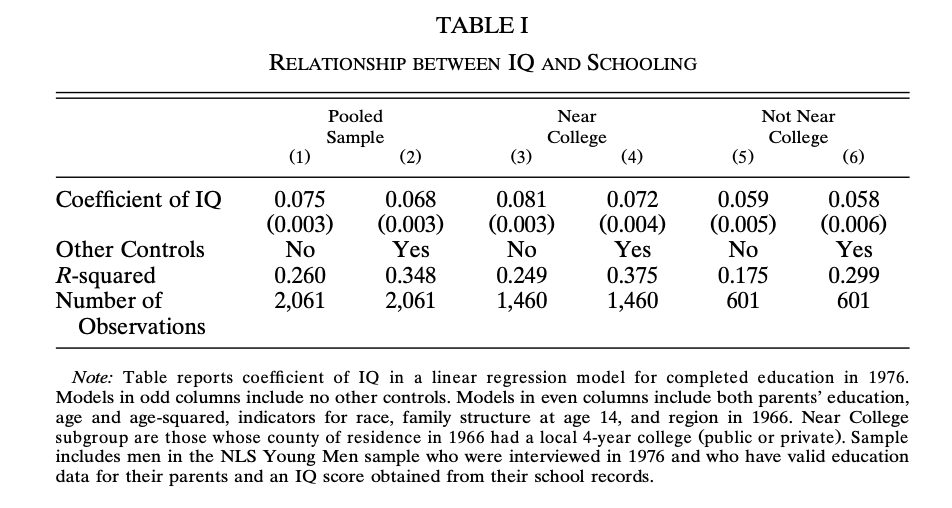
\includegraphics[scale= .5]{Table1.png}
    \end{figure}
    
    \begin{block}{Conclusion}
    Assuming the presence of nearby college is uncorrelated with ability, \textbf{college proximity is a potential IV for schooling}. 
     
    \end{block}
\end{frame}


\subsection{Alternatives to IV}
\begin{frame}{Alternatives to IV}
    \begin{itemize}
        \item Control Function Approach(Garen, 1984).
        \begin{block}{Basic Idea}
        Make some assumptions about the nature of the covariances between the unobserved ability components $a_{i}$ and $b_{i}$ and the observable variables $S_{i}$ and $Z_{i}$, and include additional terms in the earnings model that capture these relationships.
        \end{block}
        
        \item Assume mean-independence between unobserved ability and taste components and Z; also, he conditional expectations of the unobserved ability components $a_{i}$ and $b_{i}$ are linear in the schooling residual:
        \begin{equation}\tag{8a}
           \mathbb{E}[(b_{i}-\bar{b})~|~S_{i},Z_{i}]= \psi_{0}\xi_{i}, 
        \end{equation}
        \begin{equation}\tag{8b}
           \mathbb{E}[a_{i}~|~S_{i},Z_{i}]= \lambda_{0}\xi_{i}. 
        \end{equation}
    \end{itemize}
\end{frame}


\begin{frame}{}
  Together with eqaution (5), this equations imply that
  \begin{equation*}
      \mathbb{E}[log~y_{i}~|~Z_{i}]=a_{0}+\bar{b}S_{i}-\frac{1}{2}k_{1}S_{i}^{2} + \lambda_{0}\xi_{i} + \psi_{0}\xi_{i}S_{i}
  \end{equation*}
 
 This equation can be estimated by a two-step procedure in which the estimated residual \hat{\xi_{i}} from the reduced form schooling equation is substituted for $\xi_{i}$, and is substituted for $\xi_{i}$, $\hat{\xi_{i}}S_{i}$ is substituted for $\xi_{i}S_{i}$.
 
 \begin{itemize}
     \item Assumption (8a) IS PROBLEMATIC! Why?
     \begin{itemize}
         \item $Cov[b_{i},\xi_{1}~|~Z_{i}]$ and $Var[\xi_{i}~|~Z_{i}]$ potentially vary with $Z_{i}$
     \end{itemize}
     \item A simple extension of the control function approach may be appropiate if $Z_{i}$ is an indicator variable. Remember the college proximity idea?
     \item Taking this into account, and with some algebraic manipulation of equations (8a), (8b) then 
     \begin{align*}
      \mathbb{E}[log~y_{i}~|~Z_{i}] & =a_{0}+\bar{b}S_{i}-\frac{1}{2}k_{1}S_{i}^{2} + \lambda_{00}\xi_{i} + (\lambda_{01}-\lambda_{00})Z_{i}\xi_{i} + \psi_{00}\xi_{i}S_{i} \\      & + (\psi_{01}-\psi_{00})Z_{i}S_{i}\xi_{i}
  \end{align*}
 \end{itemize}
\end{frame}

\begin{frame}{A more radical approach}
Maximum likelihood estimation of a structural model of earnings and schooling, based on a complete specification of the unobservable components in the earnings function and the utility function.

\begin{block}{Edge}
An advantage of this approach is that the earnings function can be made quite general; for example, by allowing the returns to different years of schooling to vary in a flexible manner with individual ability. 
\end{block}
    
\end{frame}

\subsection{What Does IV Estimate?}
\begin{frame}{What Does a Conventional IV Estimate?}
Suppose that: 
\begin{itemize}
    \item A given individual would have schooling level $S_{i}^{c}$ and earning $y_{i}^{c}$ if he or she attended regular school system. 
    \item If he or she attended a reformed school, then the individual would have a schooling outcome of $S_{i}^{c} + \Delta S_{i}$
\end{itemize}

Let $\beta \equiv$ individual $i$'s marginal return to schooling. Then the effect of schooling reform on earnings for individual $i$ is
\begin{equation*}
    \Delta log~y_{i}= \beta_{i}\cdot \Delta S_{i}
\end{equation*}

Implying, 
\begin{align*}
   (\ast)~~ plim~b_{IV}~= \frac{Cov[log~y_{i},Z_{i}]}{Cov[S_{i},Z_{i}]} & = \frac{\mathbb{E}[log~y_i~|~Z_{i}=1]-\mathbb{E}[log~y_{i}~|~Z_{i}=0]}{\mathbb{E}[S_{i}~|~Z_{i}=1]-\mathbb{E}[S_{i}~|~Z_{i}=0]}\\
    & = \frac{\mathbb{E}[\beta_{i}\cdot \Delta S_{i}]}{\mathbb{E}[\Delta S_{i}]}
\end{align*}
\end{frame}

\begin{frame}{}
\begin{block}{Note: }
If marginal return to schooling and treatment of schooling ($\Delta S_{i}$), then the IV estimator is a consistent estimate of the avg. marginal return to eduction $\bar{\beta}=\mathbb{E}[\beta_{i}]$
\end{block}

\begin{itemize}
    \item An IV procedure based on a school reform that leads to bigger changes in the education choices of people with relatively high marginal returns to education will tend to produce an over-estimate of the average marginal return to education.
    \item Important to reconsider that the effects of a supply-side change that causes a porportional reduction in MC(S). This induced change is represented by
    \begin{equation*}
        \Delta S_{i}= r_{i}\frac{1-\theta}{k}= \bar{r}\frac{(1-\theta)}{k} + \eta_{i}\frac{(1-\theta)}{k}>0
    \end{equation*}
    Thus, the monoticity assumption required for LATE is satisfied. 
\end{itemize}   
    
\end{frame}

\begin{frame}{}
Then, individual $i$'s marginal return to schooling (in the absence intervention) is
\begin{equation*}
    \beta_{i}= \bar{\beta} + (b_{i}-\bar{b})(\frac{1-k_{1}}{k}) + \eta_{i}\frac{k_{1}}{k}
\end{equation*}
    Susbtituting in equation ($\ast$), 
    \begin{equation*}
        plim ~b_{IV}= \bar{\beta} + \Bigg[ \sigma_{\eta}^{2} \frac{k_{1}}{k} + \frac{\sigma_{b \eta}}{\bar{r}}(\frac{1-k_{1}}{k})\Bigg]
    \end{equation*}
    
Two features are worth noticing: 
\begin{enumerate}
    \item The probability limit of the IV estimator is unaffected by classical measurement error in schooling. 
    \item The validity of a particular IV estimator depends crucially on the assumption that the instruments are uncorrelated with other latent characteristics of individuals that may affect their earnings.
\end{enumerate}
\end{frame}





\section{IV Estimates of the Return to Schooling}
\begin{frame}{IV Estimates of the Return to Schooling}
\begin{figure}
    \centering
    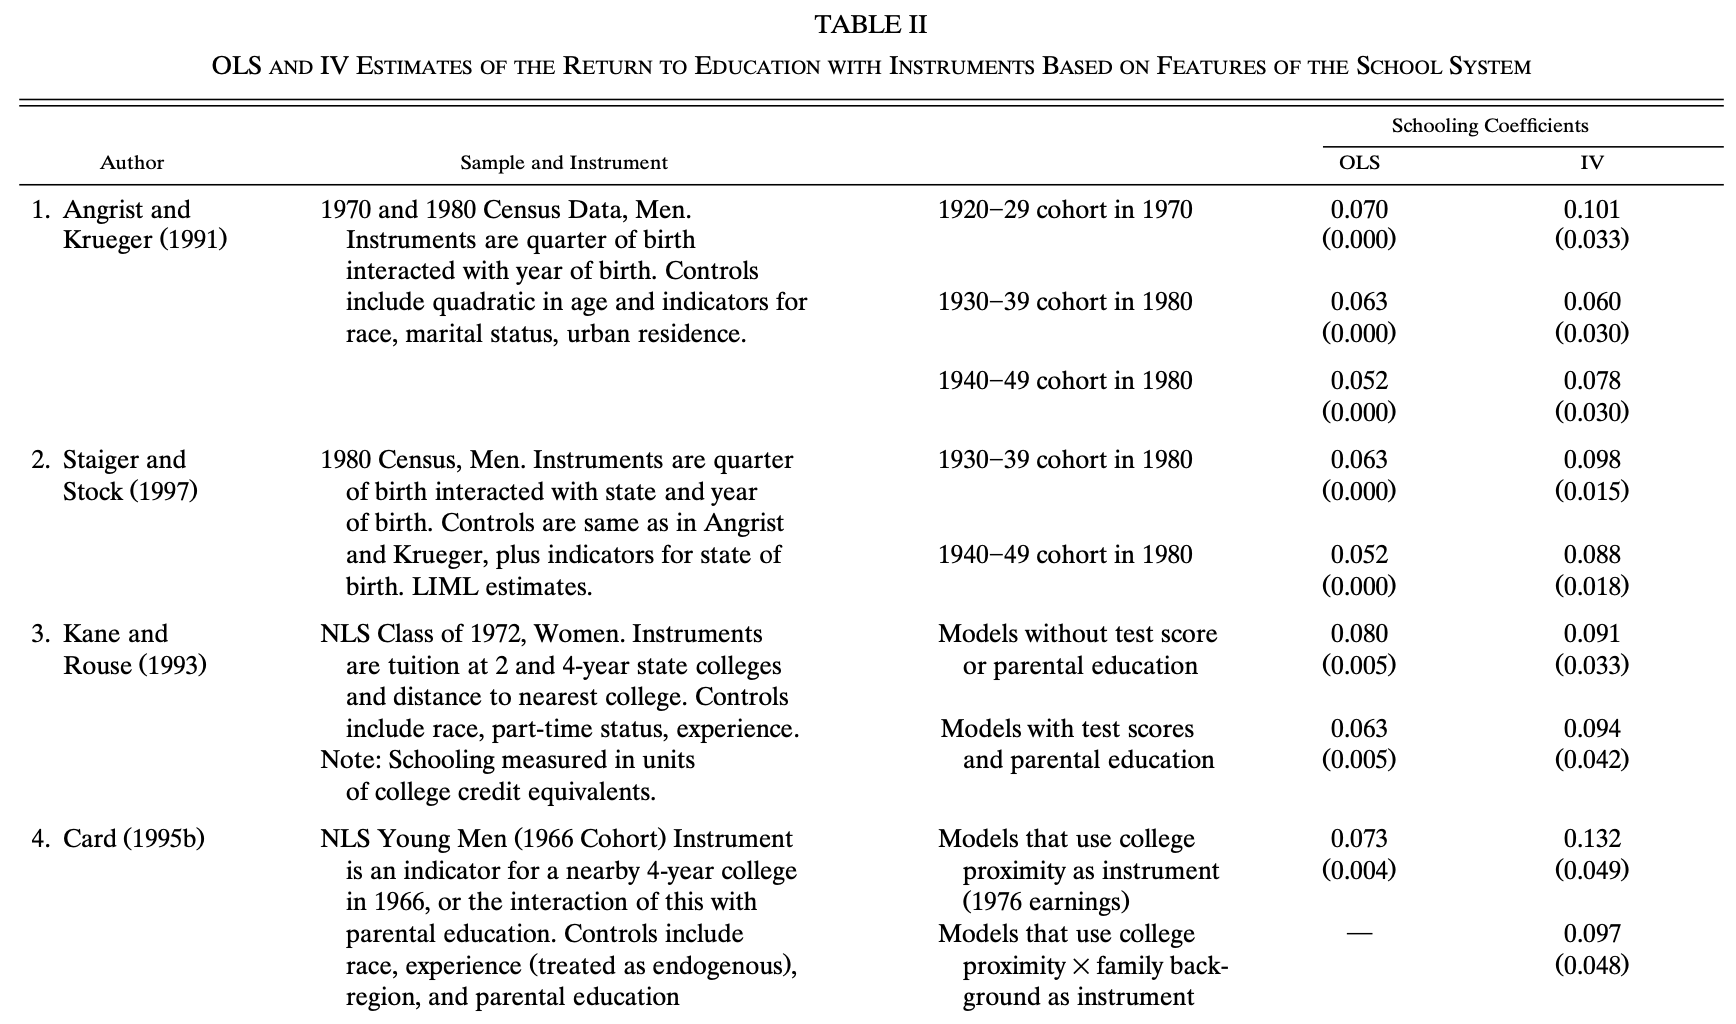
\includegraphics[scale= .42]{Table2.1.png}
\end{figure}
\end{frame}  


\begin{frame}{}
\begin{figure}
    \centering
    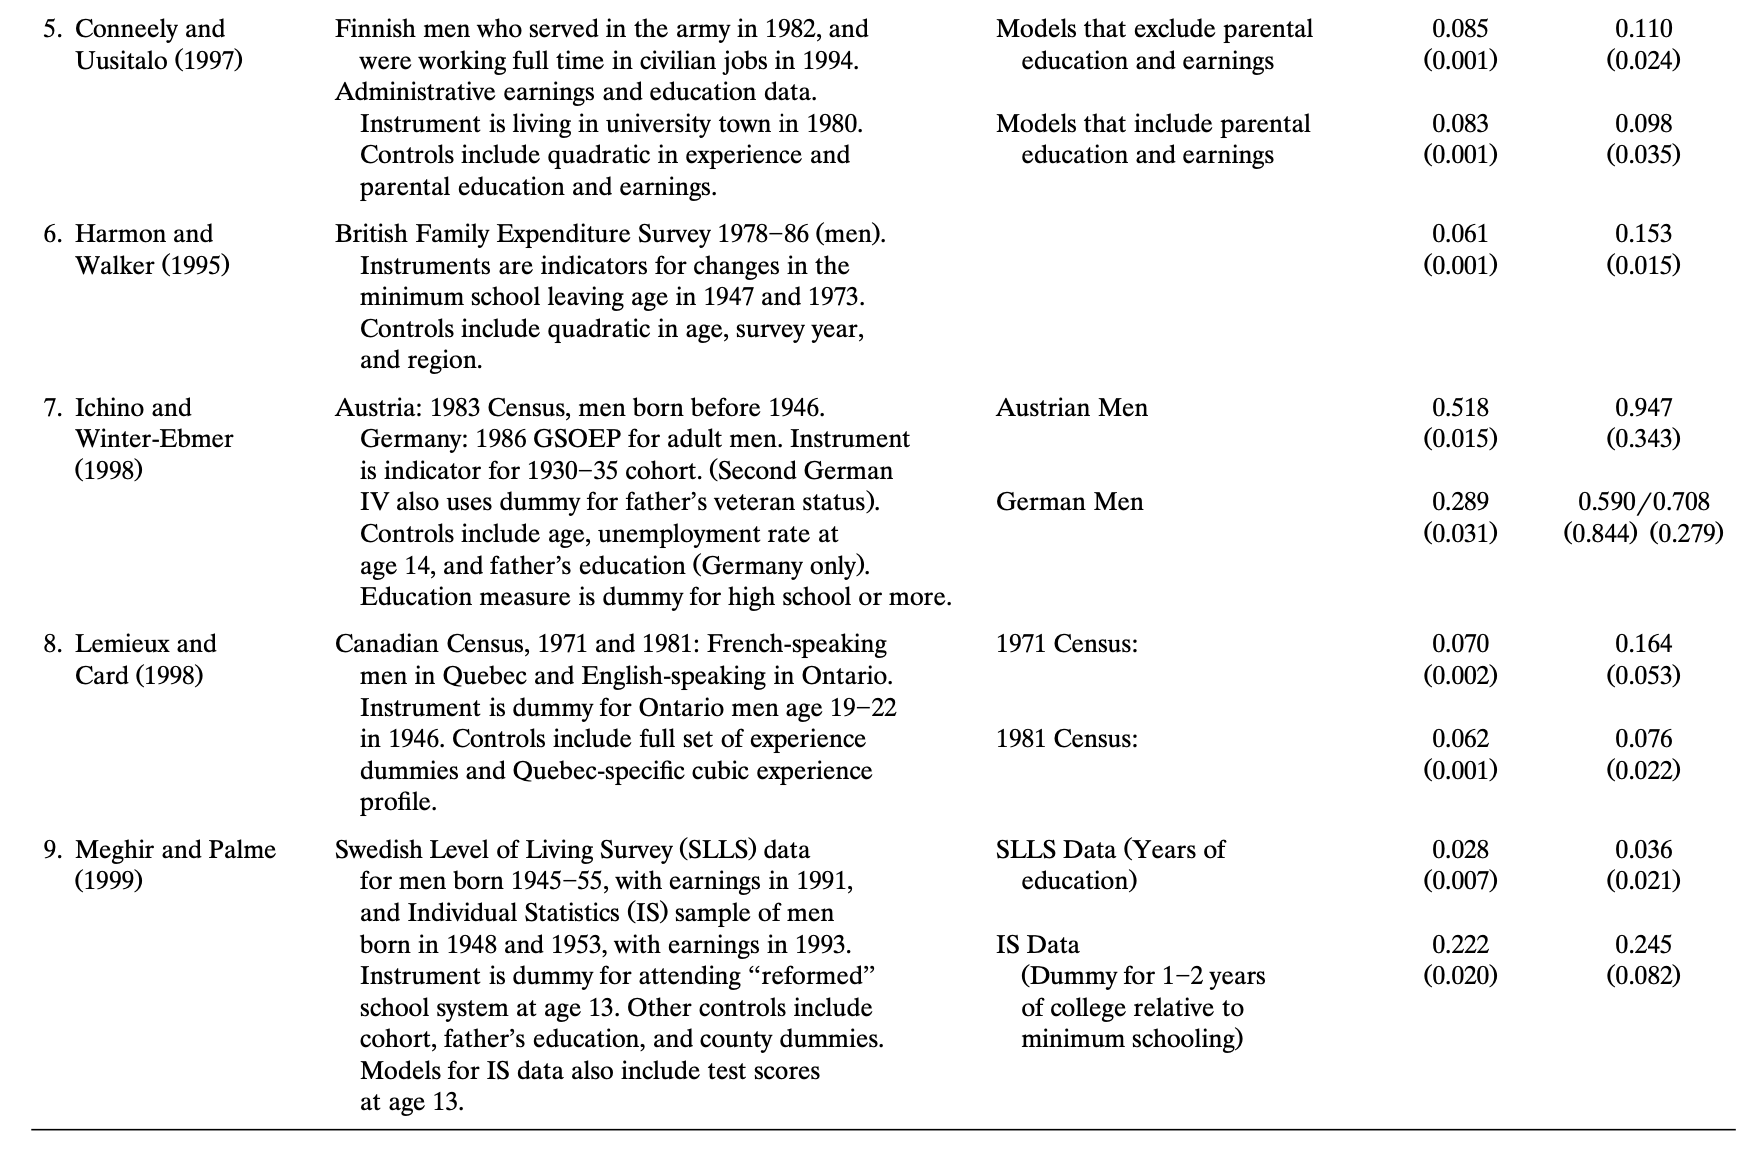
\includegraphics[scale= .4]{Table2.2.png}
\end{figure}
\end{frame}  

\begin{frame}{}
\begin{figure}
    \centering
    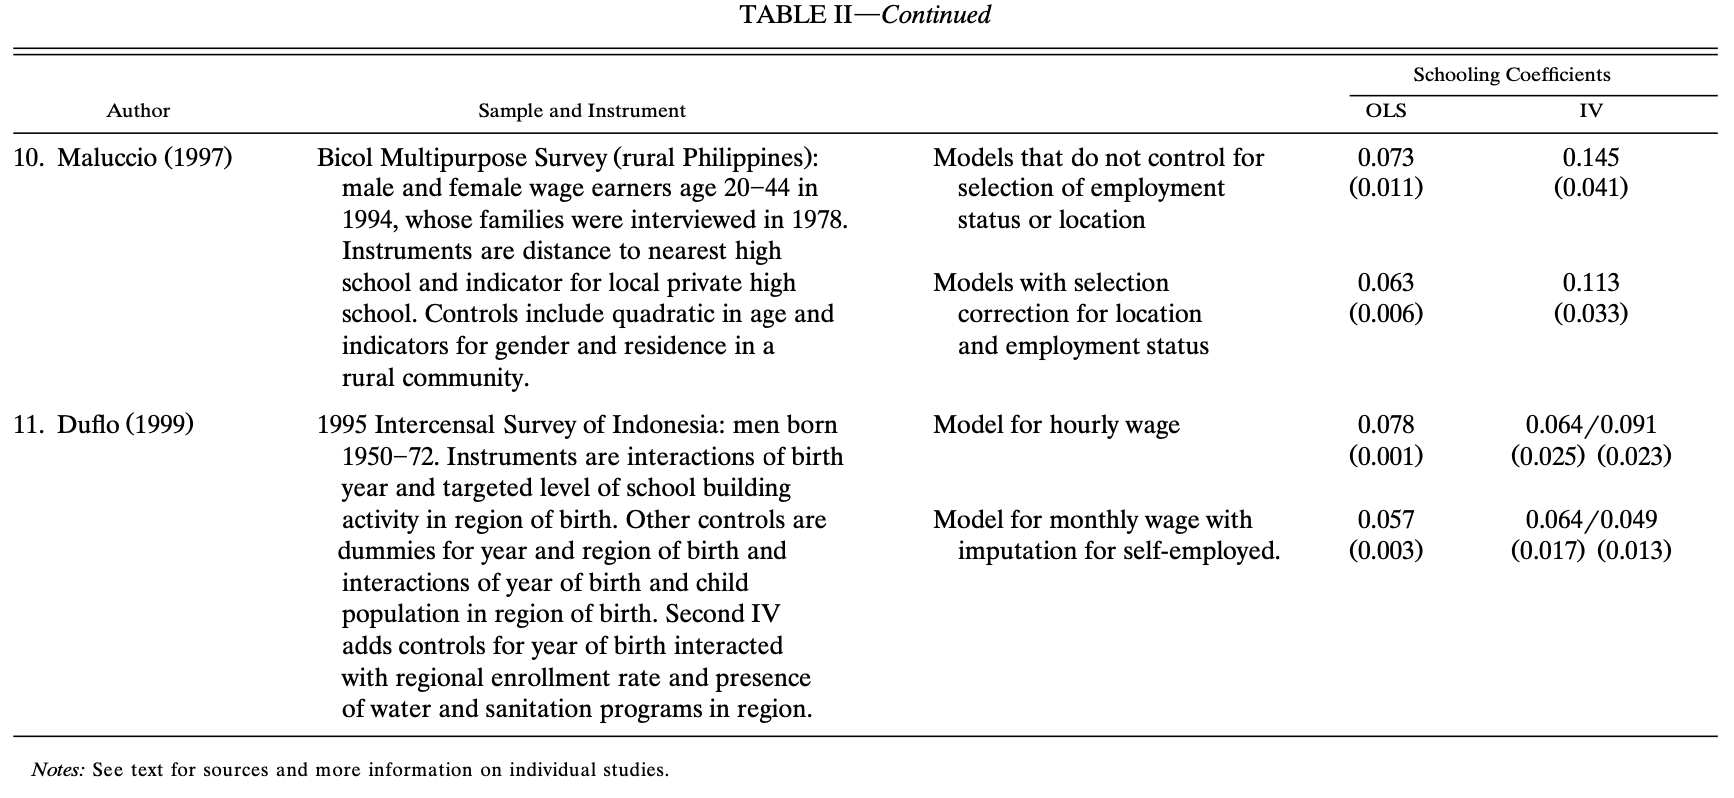
\includegraphics[scale= .4]{Table2.3.png}
\end{figure}
\end{frame} 

\section{Conclusions}
\begin{frame}{Conclusions}
   \begin{itemize}
       \item We have attempted to measure the causal effect of education on labor market earnings by using institutional features on the supply side of the education system as exogenous determinants of schooling outcomes. 
       \item Card believes it is helpful to place the returns to education literature in a standard \say{supply and demand} framework, which leads to a somewhat richer econometric model for schooling and earnings than is usually adopted in the applied literature.
       \begin{block}{NOTE: }
       Different individuals finish their schooling at a point where the marginal return to the last unit of education may be either above or below the average marginal return in the population as a whole.
       
       \end{block}
   \end{itemize} 
\end{frame}


\begin{frame}{Conclusions}
   \begin{itemize}
       \item IV estimation will typically recover a weighted avg. of returns to education for people whose choices were affected by the instrument, rather than the marginal return to education in the population. 
       \item IV estimates of the return to schooling that are at least as big and sometimes substantially bigger than the corresponding OLS estimates.
       \item In many cases the IV estimates are relatively imprecise, and none of the empirical strategies is based on true randomization. 
       \begin{itemize}
           \item Thus, no individual study is likely to be decisive in the debate over the magnitude of ability biases in OLS estimates of the return to schooling.
       \end{itemize}
       \item Seems that Griliches' (1977) assessment was spot on.
   \end{itemize} 
   
\end{frame}
\section{Bibliography}
\begin{frame}{Bibliography}
    \begin{itemize}
        \item Card, David. \say{Estimating the return to schooling: Progress on some persistent econometric problems}. \textit{Econometrica} 69, no. 5 (2001): 1127-1160.
    \end{itemize}
\end{frame}

\end{document}